% acl_report.tex — AI Strategic Framing Study
% Bocconi University · Language Technology 2026
% Compile: pdflatex acl_report && bibtex acl_report && pdflatex acl_report && pdflatex acl_report

\documentclass[11pt,a4paper,twocolumn]{article}

% ── Geometry (ACL-approximate) ────────────────────────────────────────────────
\usepackage[a4paper,
            top=2.5cm, bottom=2.5cm,
            left=1.9cm, right=1.9cm,
            columnsep=0.5cm]{geometry}

% ── Fonts and encoding ────────────────────────────────────────────────────────
\usepackage{times}
\usepackage[T1]{fontenc}
\usepackage[utf8]{inputenc}
\usepackage{microtype}

% ── Tables ───────────────────────────────────────────────────────────────────
\usepackage{booktabs}
\usepackage{multirow}
\usepackage{array}

% ── Math, graphics, misc ─────────────────────────────────────────────────────
\usepackage{amsmath}
\usepackage{graphicx}
\usepackage{caption}
\usepackage{xcolor}
\usepackage{enumitem}
\usepackage[hidelinks]{hyperref}

% ── Bibliography ──────────────────────────────────────────────────────────────
\usepackage[round,authoryear]{natbib}
\bibliographystyle{plainnat}

% ── Section formatting ────────────────────────────────────────────────────────
\usepackage{titlesec}
\titleformat{\section}{\normalfont\large\bfseries}{\thesection}{1em}{}
\titleformat{\subsection}{\normalfont\normalsize\bfseries}{\thesubsection}{1em}{}
\titlespacing*{\section}{0pt}{7pt}{3pt}
\titlespacing*{\subsection}{0pt}{5pt}{2pt}

% ── Caption style ─────────────────────────────────────────────────────────────
\captionsetup{font=small, labelfont=bf, skip=4pt}

% ── Paragraph spacing ─────────────────────────────────────────────────────────
\setlength{\parindent}{0.5em}
\setlength{\parskip}{1pt}

% ─────────────────────────────────────────────────────────────────────────────
\title{\textbf{Strategic Framing of Artificial Intelligence:\\
               A Cross-Context Corpus Study}}

\author{Anonymous Authors\\
        Bocconi University — Language Technology 2026}

\date{}
% ─────────────────────────────────────────────────────────────────────────────

\begin{document}
\maketitle

% ── Abstract ─────────────────────────────────────────────────────────────────
\begin{abstract}
AI industry actors communicate simultaneously with investors, regulators, and
the general public — yet whether they strategically adapt their framing of AI
across these audiences remains empirically untested. We present a cross-context
framing analysis of 5,946 documents from 16 major actors spanning commercial,
policy, and public communication contexts. We define five binary framing
dimensions and label 63,546 sentences using Claude Haiku, achieving
inter-annotator agreement $\kappa = 0.86$. OLS regressions on
document-level framing proportions confirm that context significantly predicts
all three framing DVs ($p < 0.001$, H1 confirmed): policy documents carry 13.6
percentage points more regulation framing than commercial documents. Satya
Nadella's policy communications contain 27.1 percentage points more innovation
framing than his commercial baseline — the largest individual strategic
adaptation signal in the corpus (H2 partially confirmed). These results
demonstrate that AI discourse is a strategic communication tool shaped by
audience, institutional role, and actor identity.
\end{abstract}

% ─────────────────────────────────────────────────────────────────────────────
\section{Introduction}
% ─────────────────────────────────────────────────────────────────────────────

When Sam Altman testified before the US Senate Judiciary Committee in May~2023,
he emphasized existential risk and the need for regulation. Speaking at a
startup conference weeks later, he emphasized transformative economic opportunity.
The same actor, the same technology, two radically different framings — chosen
for different audiences.

\textbf{Framing} is the selective emphasis of certain aspects of a topic to
promote a specific interpretation \citep{entman1993framing, goffman1974frame}.
We test whether AI actors adapt their framing strategically across three
communication contexts: commercial (investors and customers), policy (regulators
and legislators), and public (general audiences).

\textbf{Research question.} To what extent do actors adapt their framing of AI
across commercial, policy, and public contexts, controlling for time, platform,
and actor type?

\begin{description}[leftmargin=1.5em, itemsep=1pt, topsep=2pt]
  \item[H1] Context significantly predicts framing ($\beta_{\text{context}} \neq 0$).
  \item[H2] Commercial contexts increase innovation framing; policy contexts
            increase risk and regulation framing.
  \item[H3] Individual actors show greater cross-context framing variance than
            institutions.
\end{description}

We make three contributions: (1) a 5,946-document cross-context AI framing
corpus spanning 16 actors and three communication contexts; (2) a validated
five-frame annotation scheme with $\kappa = 0.86$; and (3) OLS regression
evidence that context, actor positioning, and platform independently and
significantly predict framing proportion.


% ─────────────────────────────────────────────────────────────────────────────
\section{Related Work}
% ─────────────────────────────────────────────────────────────────────────────

\citet{entman1993framing} defines framing as the selection and salience of
particular aspects of reality to promote a specific interpretation.
\citet{goffman1974frame} grounds this in communicative interaction: frames are
organizational structures actors deploy to define situations for specific
audiences. \citet{chong2007framing} extend this to strategic political
communication, showing that actors choose frames to maximize persuasive impact
on targeted audiences — the theoretical foundation for H2 and H3.

\citet{card2015media} demonstrate that frame categories can be annotated at
sentence level with reliable inter-annotator agreement across policy issues;
their corpus is the closest methodological precedent for our design. We extend
their approach to a cross-actor, multi-context setting and focus specifically
on strategic adaptation rather than static framing prevalence.

\citet{fast2017long} analyze 30 years of AI coverage in the \textit{New York
Times}, finding systematic shifts from optimistic to cautious framing as
research milestones accumulate. We complement this longitudinal view with a
cross-actor design that isolates deliberate strategic variation within a single
time window. \citet{gilardi2023chatgpt} show that LLMs match or exceed
crowd-worker annotation quality; we extend this finding to a technical domain
with expert-level frame definitions, validating against a human gold set and
three alternative models.


% ─────────────────────────────────────────────────────────────────────────────
\section{Data}
% ─────────────────────────────────────────────────────────────────────────────

\subsection{Corpus Design}

We select 16 actors spanning the full range of AI discourse: six CEOs (Sam
Altman, Dario Amodei, Jensen Huang, Satya Nadella, Mark Zuckerberg, Demis
Hassabis), six companies (OpenAI, Anthropic, Google DeepMind, Meta AI,
Microsoft, Nvidia), and four government policymakers (EU Commission, US Congress,
UK DSIT, White House OSTP). Each individual is paired with their own company
to enable direct individual-vs-institution comparison for H3. Elon Musk was
excluded after only 21 accessible documents were found (xAI blocked by
Cloudflare; no policy corpus); Satya Nadella replaces him with full
three-context coverage.

We assign each actor a \textbf{positioning} value — \textit{capability}
(Altman, Nadella, Zuckerberg, OpenAI, Meta AI, Microsoft), \textit{safety}
(Amodei, Hassabis, Anthropic, Google DeepMind), \textit{infrastructure}
(Huang, Nvidia), or \textit{regulator} (all four policymakers) — to test
whether institutional identity predicts framing beyond context in Model~3.

\subsection{Collection and Corpus Statistics}

We build a Python scraping pipeline with \texttt{requests} and
\texttt{BeautifulSoup} across 30+ source types: company blogs, arXiv
(author-name queries), government archives, podcast transcripts, and the
Wayback Machine CDX API (for sites blocked or deleted from the live web).
We manually ingest 21 PDFs via \texttt{pdfplumber}. After URL-based
deduplication, we apply five sentence-level quality filters
(non-English, length $<$8 words, JSON/HTML fragments, no AI-keyword relevance,
off-topic patterns) that reduce 208,320 raw sentences to 63,546 clean
sentences (30.5\% retained).

Table~\ref{tab:corpus} shows the final corpus of 5,946 documents.
The public context reaches only 4.0\% (target $\geq$15\%): YouTube captions
are disabled for all 14 targeted CEO videos, podcast platforms use
JavaScript rendering, and conference transcripts are paywalled — a structural
ceiling, not a sampling choice. Company documents represent 52.3\% because
$\sim$1{,}300 arXiv papers are classified as commercial (official
company-authored research output), inflating company share.

\begin{table}[t]
\centering
\caption{Final corpus distribution (N~=~5,946 documents).}
\label{tab:corpus}
\small
\begin{tabular}{lrr}
\toprule
\textbf{Context} & \textbf{Docs} & \textbf{Share} \\
\midrule
Commercial       & 3,661  & 61.6\%  \\
Policy           & 2,048  & 34.4\%  \\
Public           &   237  &  4.0\%  \\
\midrule
\textbf{Total}   & \textbf{5,946} & \textbf{100\%} \\
\midrule[0.3pt]
\multicolumn{3}{l}{\small\textit{Actor type}} \\
Company          & 3,111  & 52.3\%  \\
Policymaker      & 1,704  & 28.7\%  \\
Individual       & 1,122  & 18.9\%  \\
\bottomrule
\end{tabular}
\end{table}


% ─────────────────────────────────────────────────────────────────────────────
\section{Annotation}
% ─────────────────────────────────────────────────────────────────────────────

\subsection{Frame Definitions}

We define five binary framing dimensions derived from the computational
framing literature \citep{card2015media} plus a \textsc{None} label.
Each sentence receives one or more labels, or \textsc{None} if no frame
is explicitly stated in the text (inferred frames are coded \textsc{None}).

\vspace{3pt}
\noindent\textit{Innovation/Progress}: AI as transformative, with an explicit claim about societal benefit or scientific advance.
\textit{Economic Benefit}: explicit claim about jobs, revenue, productivity, or national competitiveness.
\textit{Risk/Harm}: concrete near-term harms — bias, job loss, misuse, or surveillance.
\textit{Regulation/Governance}: explicit institutional mechanism — law, framework, oversight body.
\textit{Existential/AGI}: long-term civilizational risk, AGI, or superintelligence.
\vspace{3pt}

Full definitions and edge-case rules are in \texttt{docs/annotation\_guidelines.md}.

\subsection{Inter-Annotator Agreement}

Two annotators independently label a stratified 100-sentence overlap set
(balanced across contexts and actors), measuring Cohen's $\kappa$
\citep{landis1977measurement} with a $\kappa \geq 0.70$ gate before corpus-scale
labeling.

\begin{table}[t]
\centering
\caption{Inter-annotator agreement by annotation round.}
\label{tab:kappa}
\small
\begin{tabular}{clcp{3.2cm}}
\toprule
\textbf{Round} & \textbf{$\kappa$} & \textbf{Result} & \textbf{Root cause} \\
\midrule
1 & 0.36 & FAIL & None/frame boundary underspecified \\
2 & 0.37 & FAIL & Corpus noise \\
3 & 0.86 & PASS & Clean sentence pool \\
\bottomrule
\end{tabular}
\end{table}

Rounds~1 and~2 fail despite guideline revision after Round~1.
Diagnostic analysis reveals that 24 of 28 Round~2 disagreements trace to
identical problematic sentences: React/Next.js JSON fragments, FEMA boilerplate,
three-word header fragments, and economic statistics with no AI content. We
apply five quality filters (§3.2) to remove 144,774 sentences, redraw the
overlap set from the clean pool, and run Round~3, achieving $\kappa = 0.86$
across all six label categories (Table~\ref{tab:kappa}). The single-round
jump confirms that early failures reflect corpus noise, not genuine annotation
ambiguity.

\subsection{LLM Labeling and Validation}

We label all 63,546 sentences using \texttt{claude-haiku-4-5-20251001} via the
Anthropic Messages API, using a system prompt derived directly from the
annotation guidelines (batch size 15, 0.3-second inter-call delay).
We validate against the 100-sentence human gold set: macro precision~=~0.847,
recall~=~0.534, F1~=~0.633. High precision indicates that when Haiku assigns
a frame, it is almost always correct; low recall indicates it defaults to
\textsc{None} for $\sim$47\% of true positives. Framing scores are therefore
systematic underestimates — positive findings are \emph{conservative}, not
inflated. Three alternative models confirm the same conservative bias pattern:
GPT-4o-mini F1~=~0.472, Llama~3.3-70B F1~=~0.415, Gemini~2.5-Flash F1~=~0.214.
Haiku achieves the highest F1 of any tested model.

\subsection{Dependent Variable Selection}

We exclude two frames as regression DVs. \textbf{Economic Benefit} has LLM
recall~=~0.00 in the policy context, making any coefficient an artifact of
annotation failure rather than real framing. \textbf{Existential/AGI} reaches
only 1.1\% sentence frequency with near-zero document-level variance. The three
retained DVs — \textit{innovation\_score}, \textit{risk\_score},
\textit{regulation\_score} — have frequencies of 18.7\%, 8.7\%, and 11.5\%
and non-zero LLM recall in every context.


% ─────────────────────────────────────────────────────────────────────────────
\section{Results}
% ─────────────────────────────────────────────────────────────────────────────

For each document $d$ and frame $F$:
$\text{score}_{F,d} = (\text{sentences labeled } F \text{ in } d) /
(\text{total sentences in } d)$.
This proportion normalizes framing density by document length. Documents with
fewer than 5 sentences are excluded (3,411 removed), yielding $N = 2{,}535$
documents for regression. Reference categories: context~=~commercial,
positioning~=~capability, platform~=~blog, actor\_type~=~company.

\subsection{H1: Context Predicts Framing (Model~1)}

Model~1: $\text{score}_{d} = \beta_0 + \beta_1 C(\text{context}_d) + \beta_2 \text{post\_chatgpt}_d + \varepsilon_d$.
Post-ChatGPT is a binary equal to 1 for documents dated on or after 2022-11-30,
controlling for corpus-wide discursive intensification after the public launch of ChatGPT.

\textbf{H1 is confirmed.} Table~\ref{tab:m1} shows that context is a significant
predictor of all three DVs. Policy documents carry 13.6~pp more regulation
framing than commercial ($\beta = +0.136$, $p < 0.001$), explaining 12.1\% of
regulation variance. Risk framing peaks in policy (+5.5~pp) and drops in public
settings ($-4.3$~pp). Innovation is significantly lower in policy than
commercial ($-2.3$~pp, $p = 0.016$), confirming commercial as the innovation
register by inversion. Post-ChatGPT intensification is significant for
innovation ($+4.8$~pp) and regulation ($+2.3$~pp), reflecting a corpus-wide
discursive shift after November~2022. The low $R^2$ for innovation (0.014)
reveals substantial actor-level heterogeneity that requires Model~2.

\begin{table}[t]
\centering
\caption{Model~1 OLS results ($N = 2{,}535$). Coefficients are pp changes
relative to commercial baseline. SE in parentheses.
${}^{***}{<}0.001$, ${}^{**}{<}0.01$, ${}^{*}{<}0.05$.}
\label{tab:m1}
\small
\setlength{\tabcolsep}{4pt}
\begin{tabular}{lrrr}
\toprule
\textbf{Predictor} & \textbf{Innov.} & \textbf{Risk} & \textbf{Reg.} \\
\midrule
Policy
  & $-$0.023$^{*}$ & $+$0.055$^{***}$ & $+$0.136$^{***}$ \\
  & (0.009)        & (0.006)          & (0.008) \\
Public
  & $+$0.036       & $-$0.043$^{***}$ & $-$0.017 \\
  & (0.019)        & (0.012)          & (0.016) \\
Post-ChatGPT
  & $+$0.048$^{***}$ & $+$0.002       & $+$0.023$^{**}$ \\
  & (0.009)          & (0.006)        & (0.007) \\
\midrule
$R^2$ & 0.014 & 0.041 & 0.121 \\
\bottomrule
\end{tabular}
\end{table}

\subsection{H2: Strategic Adaptation (Model~2)}

Model~2 adds actor fixed effects and actor$\times$context interactions. A
significant positive interaction means the actor frames more intensely in that
context than actor-level and context-level effects alone predict — the
operational definition of strategic adaptation.

Model~2 requires $\geq$50 documents per actor$\times$context cell and presence
in $\geq$2 contexts. Three actors qualify: Microsoft (comm $n=84$, pol $n=152$),
OpenAI (comm $n=194$, pol $n=81$), and Satya Nadella (comm $n=59$, pol $n=66$),
yielding $N = 636$ documents. Public context is excluded — sparse coverage
produces near-degenerate estimates.

\begin{table}[t]
\centering
\caption{Model~2: significant actor$\times$policy interactions ($N=636$).
         Reference actor: Microsoft.}
\label{tab:m2}
\small
\begin{tabular}{llrrr}
\toprule
\textbf{Actor} & \textbf{DV} & $\hat{\beta}$ & \textbf{SE} & $p$ \\
\midrule
Nadella & innovation & $+0.271$ & 0.044 & ${<}0.001^{***}$ \\
OpenAI  & innovation & $+0.101$ & 0.037 & $0.007^{**}$ \\
\midrule
OpenAI  & regulation & $-0.097$ & 0.023 & ${<}0.001^{***}$ \\
OpenAI  & risk       & $-0.056$ & 0.028 & $0.046^{*}$ \\
\bottomrule
\end{tabular}
\end{table}

\textbf{H2 is partially confirmed.} Table~\ref{tab:m2} shows four significant
interactions. Satya Nadella's policy documents contain 27.1~pp more innovation
framing than his commercial baseline plus the average policy shift predicts
($\beta = +0.271$, $p < 0.001$) — the strongest strategic adaptation signal
in the corpus. When addressing regulators, Nadella foregrounds AI as an
innovation driver rather than a governance challenge. OpenAI increases
innovation framing in policy (+10.1~pp) while simultaneously suppressing
regulation ($-9.7$~pp) and risk ($-5.6$~pp) language, suggesting active
resistance to regulatory framing when communicating with policymakers.

The H2 innovation finding is conservative: LLM recall for Innovation/Progress
is 28~pp lower in commercial contexts (0.28) than in policy (0.56), meaning the
measured commercial$\,{>}\,$policy gap understates the true effect. Economic
Benefit is untestable given LLM recall = 0.00 in policy.

\subsection{H3: Individual vs.\ Institution Variance}

For each qualifying actor ($\geq$50 documents in $\geq$2 contexts) we compute
the standard deviation of context-level mean framing scores. Five of 16 actors
qualify.

\begin{table}[t]
\centering
\caption{Cross-context variance ($\sigma$) for qualifying actors.
         Higher $\sigma$ = greater framing adaptation across contexts.}
\label{tab:variance}
\small
\setlength{\tabcolsep}{4pt}
\begin{tabular}{llcrrr}
\toprule
\textbf{Actor} & \textbf{Type} & \textbf{Ctx} &
  \textbf{Inn.~$\sigma$} & \textbf{Risk~$\sigma$} & \textbf{Reg.~$\sigma$} \\
\midrule
Satya Nadella   & ind & 3 & \textbf{0.129} & 0.050 & \textbf{0.064} \\
Microsoft       & co  & 3 & 0.031 & 0.049 & 0.049 \\
UK DSIT         & pm  & 2 & 0.088 & 0.036 & 0.012 \\
OpenAI          & co  & 2 & 0.037 & 0.007 & 0.011 \\
Google DeepMind & co  & 2 & 0.011 & 0.032 & 0.016 \\
\bottomrule
\end{tabular}
\end{table}

\textbf{H3 is directionally supported but not formally testable.}
Satya Nadella — the sole qualifying individual — exhibits the highest
cross-context variance on innovation ($\sigma = 0.129$) and regulation
($\sigma = 0.064$), 4.2$\times$ and 1.3$\times$ higher than paired company
Microsoft (Table~\ref{tab:variance}; Figure~\ref{fig:var}). A formal $t$-test
requires $\geq$2 qualifying individuals; only 1 qualifies due to the
public-context coverage gap. We report Nadella's result as illustrative
evidence consistent with H3, with corpus limitations explicitly disclosed.
The M2 interaction ($\beta = +0.271^{***}$) and the variance analysis
($\sigma = 0.129$) are complementary views of the same pattern.

\begin{figure}[t]
  \centering
  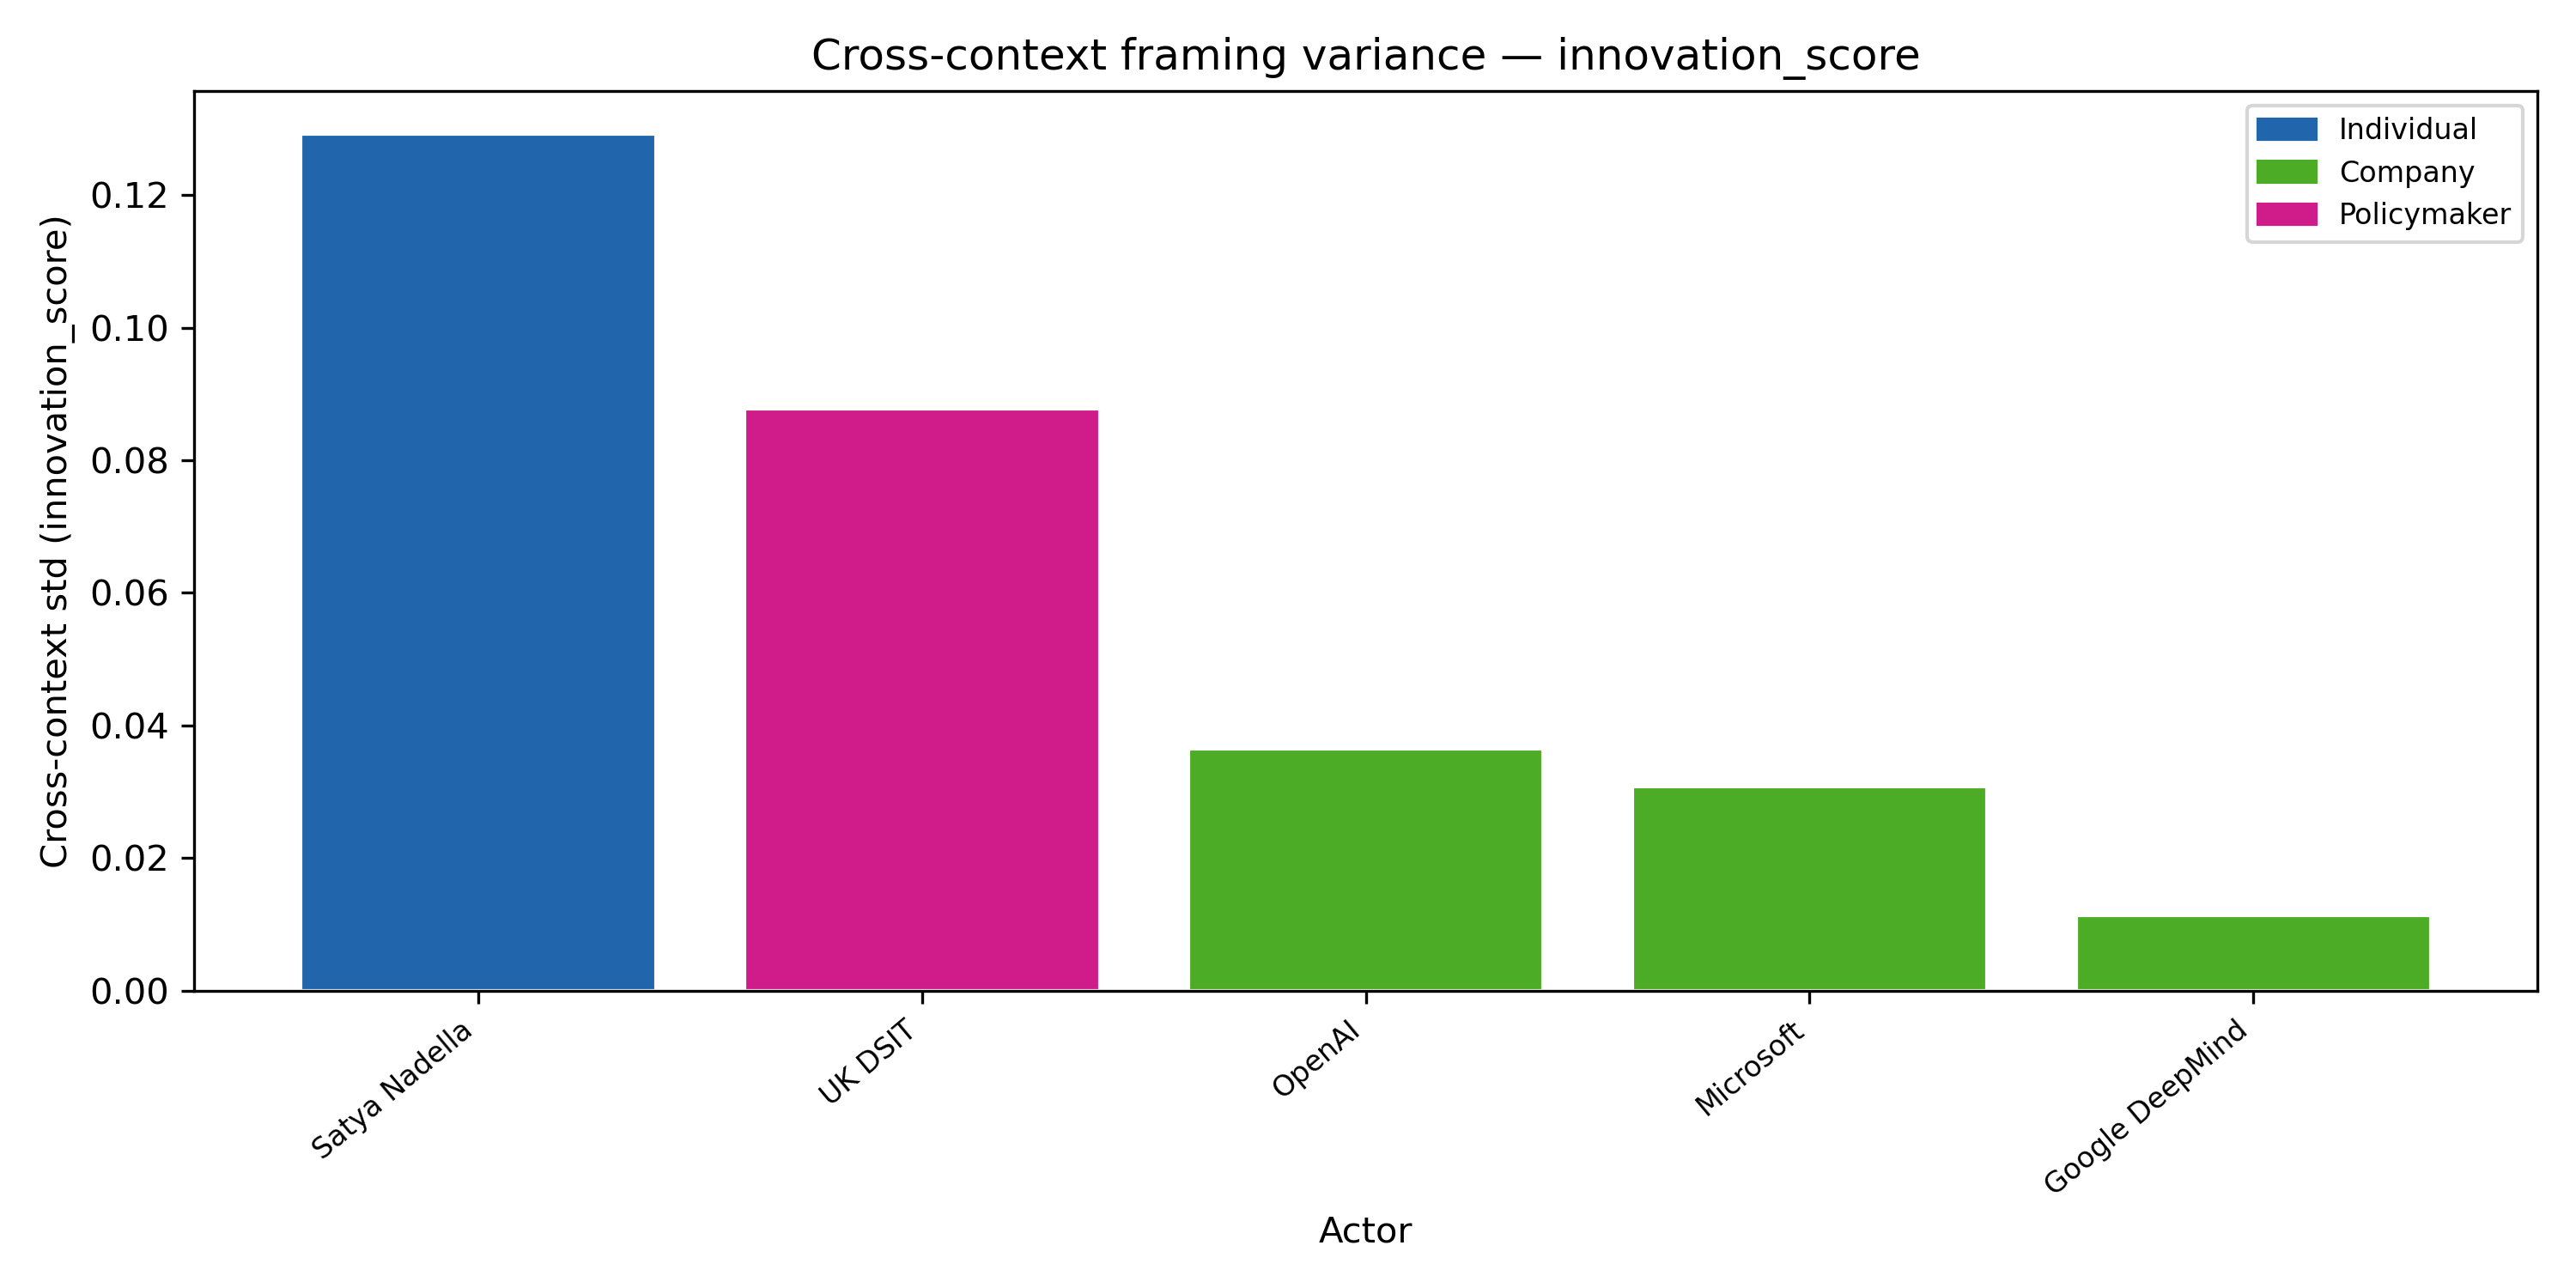
\includegraphics[width=\columnwidth]{outputs/figures/variance_innovation_score.png}
  \caption{Cross-context innovation variance for qualifying actors. Nadella
           (individual) shows substantially higher variance than all qualifying
           companies. Variance figures for risk and regulation are in
           \texttt{outputs/figures/}.}
  \label{fig:var}
\end{figure}

\subsection{Model~3: Structural Controls}

Model~3 adds actor type, positioning, platform, and time ($N = 2{,}535$).
The cluster \{policymaker, policy context, regulator positioning, testimony
platform\} is near-perfectly collinear; we report only interpretable terms.
\textit{Safety} positioning predicts less innovation framing ($\beta = -0.042$,
$p < 0.001$), more risk ($\beta = +0.038$, $p < 0.001$), and more regulation
($\beta = +0.050$, $p < 0.001$) — confirming that actors' public positioning
maps onto their linguistic output across all contexts. Speeches carry
14.5~pp more innovation framing than blogs ($\beta = +0.145$, $p = 0.006$);
research papers suppress both innovation ($\beta = -0.084$, $p < 0.001$) and
regulation framing ($\beta = -0.031$, $p = 0.007$). Regulation framing
achieves the highest explained variance across all models ($R^2 = 0.221$
in M3), driven by positioning and platform rather than context alone.


% ─────────────────────────────────────────────────────────────────────────────
\section{Discussion}
% ─────────────────────────────────────────────────────────────────────────────

Satya Nadella adapts more than any other qualifying actor: a 27.1~pp innovation
spike in policy documents signals deliberate rhetorical strategy — framing AI
as an economic opportunity rather than a governance challenge when addressing
Congress. OpenAI shows the inverse: active suppression of regulation and risk
language in policy contexts while amplifying innovation framing. Together, these
patterns suggest that commercial actors treat policy audiences as arenas for
shaping regulatory narrative toward favorable outcomes, not as targets for
safety reassurance.

Safety positioning predicts framing content independently of context: Anthropic,
Amodei, Hassabis, and Google DeepMind consistently use more risk and regulation
language regardless of setting. Institutional identity constrains — but does
not eliminate — context-driven adaptation. Actors frame strategically, but
within the space their brand positioning defines: a safety-positioned actor
does not suppress risk framing even in commercial contexts.

These findings reframe AI discourse as a strategic rather than descriptive
practice. Public deliberation about AI policy is not driven by technological
facts alone but by deliberate communication strategies tuned to audience
expectations and institutional incentives. The public-context gap prevents
formal H3 testing; richer public-context data would resolve whether individual
CEOs adapt more freely than their companies.


% ─────────────────────────────────────────────────────────────────────────────
\section{Conclusion}
% ─────────────────────────────────────────────────────────────────────────────

We study whether major AI actors strategically adapt their framing across
commercial, policy, and public communication contexts. We construct a 5,946-document
corpus, annotate 63,546 sentences with $\kappa = 0.86$, and estimate OLS
regression models on document-level framing proportions. H1 is confirmed:
context significantly predicts all three framing dimensions ($p < 0.001$). H2
is partially confirmed: policy increases risk (+5.5~pp) and regulation
(+13.6~pp) framing; Satya Nadella and OpenAI exhibit strong strategic innovation
framing in policy contexts. H3 is directionally supported but not formally
testable given that only one individual qualifies for variance analysis. Future
work should expand public-context coverage — targeted collection of conference
keynotes and formally transcribed interviews — to enable direct
individual-vs-institution hypothesis testing.


% ─────────────────────────────────────────────────────────────────────────────
\section*{Limitations}
% ─────────────────────────────────────────────────────────────────────────────

\paragraph{Public context underrepresentation.}
Public documents constitute 4.0\% of the corpus (target: $\geq$15\%). YouTube
captions are disabled for all 14 targeted CEO videos; podcast platforms use
JavaScript rendering; conference transcripts are paywalled. This structural
ceiling collapses the three-context design for most individual actors and
prevents formal H3 testing.

\paragraph{arXiv inflation.}
Company documents represent 52.3\% because $\sim$1{,}300 arXiv papers are
classified as commercial (correct: company-authored research serves the same
audience function as product blogs) but inflates company share relative to
the other actor types.

\paragraph{Actor-context sparsity.}
Twenty-four actor$\times$context pairs fall below the 50-document minimum. Model~2
is restricted to three actors (Microsoft, OpenAI, Nadella) and cannot
generalize to the full corpus. Per-actor counts appear in Appendix~A.

\paragraph{English-only corpus.}
All documents are in English. Multilingual framing variation — which may differ
systematically across regulatory jurisdictions — is outside the scope of this study.


% ─────────────────────────────────────────────────────────────────────────────
\section*{Ethical Considerations}
% ─────────────────────────────────────────────────────────────────────────────

All documents are publicly available: corporate blog posts, government
publications, official testimonies, and publicly accessible podcast transcripts.
No personal data are collected. Wayback Machine sources consist exclusively of
previously public pages recovered for academic reproducibility. The LLM is used
for annotation only, not to generate any corpus content. All annotation
guidelines, prompts, and code are released with the data.


% ─────────────────────────────────────────────────────────────────────────────
\section*{Data Availability}
% ─────────────────────────────────────────────────────────────────────────────

All code, annotation guidelines, regression outputs, and labeled data are
available at \url{https://github.com/juliavikr/ai-framing-project}. All
sources were publicly accessible at collection time. See Appendix~A for the
full per-actor source list.


% ─────────────────────────────────────────────────────────────────────────────
\bibliography{references}
% ─────────────────────────────────────────────────────────────────────────────


% ─────────────────────────────────────────────────────────────────────────────
\appendix
\section{Per-Actor Document Counts}
\label{app:actors}
% ─────────────────────────────────────────────────────────────────────────────

Table~\ref{tab:actors} reports per-actor counts in the regression dataset
($N = 2{,}535$, after the $\geq$5-sentence filter). Actors with fewer than
50 documents in a given context are excluded from Model~2 interaction analysis.
Positioning: C~=~capability, S~=~safety, I~=~infrastructure, R~=~regulator.

\begin{table}[h]
\centering
\caption{Per-actor document counts in the regression dataset (N~=~2,535).}
\label{tab:actors}
\small
\setlength{\tabcolsep}{3.5pt}
\begin{tabular}{llcrrrr}
\toprule
\textbf{Actor} & \textbf{Type} & \textbf{Pos.} &
  \textbf{Com.} & \textbf{Pol.} & \textbf{Pub.} & \textbf{Tot.} \\
\midrule
Dario Amodei    & ind & S & 310 &   2 &  3 & 315 \\
Satya Nadella   & ind & C &  59 &  66 & 36 & 161 \\
Demis Hassabis  & ind & S &  80 &   3 &  8 &  91 \\
Mark Zuckerberg & ind & C & 118 &   1 &  3 & 122 \\
Jensen Huang    & ind & I & 148 &   0 &  7 & 155 \\
Sam Altman      & ind & C &  13 &   1 &  3 &  17 \\
\midrule
Anthropic       & co  & S & 265 &   2 &  7 & 274 \\
OpenAI          & co  & C & 194 &  81 &  0 & 275 \\
Google DeepMind & co  & C & 183 &   0 & 17 & 200 \\
Meta AI         & co  & C & 170 &   0 &  0 & 170 \\
Microsoft       & co  & C &  84 & 152 & 28 & 264 \\
Nvidia          & co  & I &  78 &   0 &  3 &  81 \\
\midrule
UK DSIT         & pm  & R &   0 & 236 & 16 & 252 \\
White House OSTP& pm  & R &   0 &  63 &  0 &  63 \\
EU Commission   & pm  & R &   0 &  90 &  2 &  92 \\
US Congress     & pm  & R &   0 &   3 &  0 &   3 \\
\midrule
\textbf{Total}  & & &
  \textbf{1,702} & \textbf{700} & \textbf{133} & \textbf{2,535} \\
\bottomrule
\end{tabular}
\end{table}

\end{document}
